\subsection{Codifica del Proof of Concept}
Questa fase comincia subito dopo il termine della precedente e finisce con la data di consegna per la \textit{Revisione di Progettazione}, ovvero dal 08-02-2021 al 01-03-2021. Lo scopo di questa fase è quello di consolidare la progettazione della Techonology Baseline attraverso l'implementazione di un Proof Of Concept.
\subsubsection{Incremento I}
\paragraph{Obiettivi}
\begin{itemize}
\item Sviluppo di una prima bozza dell'\glo{UI} ;
\item Implementazione di un componente per il caricamento dei dati nel sistema attraverso un file in formato \glo{CSV} \textbf{[UC1.1.1]};
\item Implementazione di una sezione per la selezione delle dimensioni da utilizzare \textbf{[UC2]}.
\end{itemize}
		
\paragraph{Periodi e attività} \mbox{}\\\mbox{}\\
Questo incremento si compone di un unico periodo, dal 08-02-2021 al 18-02-2021, con milestone fissata per l'ultimo giorno. Comprende attività di:
\begin{itemize}
\item \textbf{Verifica dei documenti};
\item \textbf{Studio delle tecnologie:} studio della documentazione delle librerie \glo{D3.js} e \glo{React};
\item \textbf{Progettazione:} progettazione di un componente per il caricamento dei dati e uno per la selezione delle dimensioni;
\item \textbf{Codifica:} codifica dei componenti progettati;
\item \textbf{Verifica software:} verifica sulle funzionalità software aggiunte.
\end{itemize}

\subsubsection{Incremento II}  
\paragraph{Obiettivi}
\begin{itemize}
\item Implementazione della visualizzazione \glo{Scatter Plot Matrix} \textbf{[UC5.1]};
\item Aggiunta di alcuni controlli per la configurazione dei parametri relativi alla visualizzazione precedentemente implementata  \textbf{[UC6.1]}. 
\end{itemize}			
	
\paragraph{Periodi e attività} \mbox{}\\\mbox{}\\
Questo incremento si compone di un unico periodo, dal 18-02-2021 al 01-03-2021, con milestone fissata per l'ultimo giorno. Comprende attività di:
\begin{itemize}
\item \textbf{Studio delle tecnologie:} studio più approfondito della documentazione delle tecnologie interessate;
\item \textbf{Progettazione:} progettazione di un componente per la visualizzazione \glo{Scatter Plot Matrix} e del collegamento tra server, \glo{database} e \glo{web app};
\item \textbf{Codifica:} codifica del componente per la visualizzazione con relativa parametrizzazione. Integrazione con le altre tecnologie individuate durante il primo periodo per verificarne la fattibilità;
\item \textbf{Verifica software:} verifica delle funzionalità software aggiunte.
\end{itemize}

\begin{figure}[h]
	\centering	
	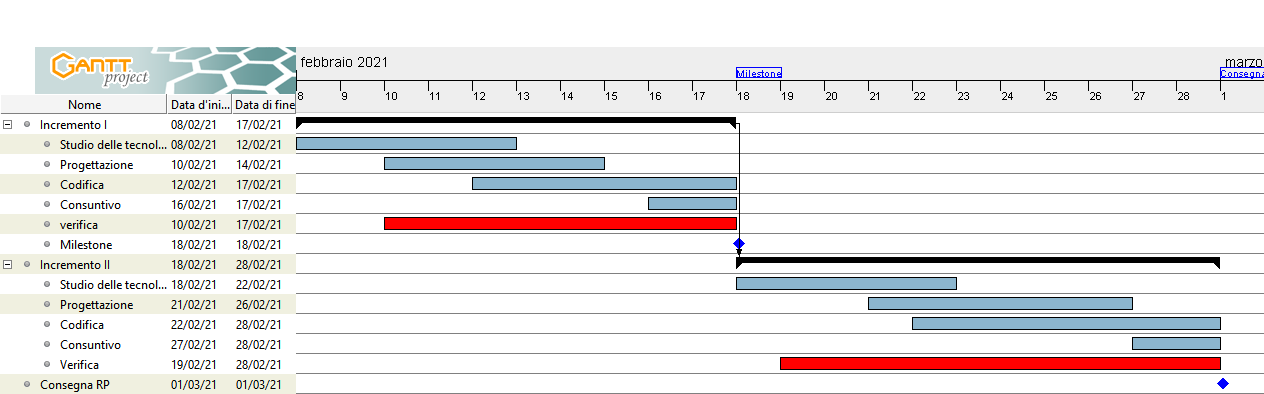
\includegraphics[width=\linewidth]{Images/GanttPianificazioneProgettazionePoc.PNG}
	\caption{Diagramma di Gantt dell'attività di progettazione e codifica del Proof Of Concept}
\end{figure}




